\documentclass{cta-author}

\newtheorem{theorem}{Theorem}{}
\newtheorem{corollary}{Corollary}{}
\newtheorem{remark}{Remark}{}

\begin{document}

\supertitle{Submission Template for IET Research Journal Papers}

\title{Title}

\author{\au{First Author$^{1}$}, \au{Second Author$^{2\corr}$}, \au{Third Author$^{3}$}}

\address{\add{1}{First Department, First University, Address, City, Country Name}
\add{2}{Second Company Department, Company Address, City, Country Name}
\add{3}{Third Department, Third University, Address, Country Name}
\add{4}{Current affiliation: Fourth Department, Fourth University, Address, Country Name}
\email{corresponding.author@second.com}}

\begin{abstract}
This should be informative and suitable for direct
inclusion in abstracting services as a self-contained
article. It should not exceed 200 words. It should
summarise the general scope and also state the main results
obtained, methods used, the value of the work and the
conclusions drawn. No figure numbers, table numbers,
references or displayed mathematical expressions should be
included. The abstract should be included in both the
Manuscript Central submission step (Step 1) and the
submitted paper.
\end{abstract}

\maketitle

\section{Introduction}\label{sec1}

This document is a template, an electronic copy of which
can be downloaded from the Research Journals Author Guide
page on the IET's Digital Library. For questions on paper
guidelines, please contact the relevant journal inbox as
indicated on each journal's website.

Before submitting your final paper, check that the format
conforms to this template and the Author Guide [1].
Specifically, check to make sure that the correct
referencing style has been used and the citations are in
numerical order throughout the text. If your paper does not
meet all of the requirements, your paper will be
unsubmitted and you will be asked to correct it.

\section{Language, spelling and grammar}\label{sec2}

All papers must be written in UK English. If English is not
your first language, you should ask an English-speaking
colleague to proofread your paper. Papers that fail to meet
basic standards of literacy are likely to be unsubmitted by
the Editorial Office.

\section{Length}\label{sec3}

Original research papers submitted to the IET Research
Journals should conform to the~IET Research Journals Length
Policy [2]. The length guidelines include the
abstract, references and appendices but do not include
figure captions, equations, or table content.

\section{Author names and affiliations}\label{sec4}

Names and affiliations should immediately follow the title.
To avoid confusion, the family name must be written as the
last part of each author name and the first name should be
spelt out rather than abbreviated (e.g. John A.K. Smith).
Author details must not show any professional title (e.g.
Managing Director), any academic title (e.g. Dr.) or any
membership of any professional organisation.

For multiple-authored articles, list the full names of all
the authors, using identifiers to link an author with an
affiliation where necessary (eg. John AK Smith$^{1}$,
Edward Jones$^{2}$).

The full affiliations of all authors should then be listed.
Affiliations should include: the department name; the name
of the university or company; the name of the city; and the
name of the country (e.g. $^{1}$Department of Electrical
Engineering, University of Sydney, Sydney, Australia).

If an author's present address is different from the
address at which the work was carried out, this should be
given as a secondary affiliation (see affiliation$^{4})$.

Only the email address of the corresponding author is
required and should be indicated with a *.

All co-authors must be listed on ScholarOne Manuscript
Central as part of the submission process. There is also
the opportunity to include ORCID IDs for all authors in
step 3 of the submission steps [3]. If you do not know
a co-author's ORCID ID there is a look-up option included
in Manuscript Central.

\section{Page Formatting}\label{sec5}

An easy way to comply with the requirements stated in the
Author Guide [1] is to use this document as a template and
simply type your text into it. PDF files are also accepted,
so long as they follow the same style.

\subsection{Page Layout}\label{subsec5.1}

Our papers are double column format; one column width is
8.6cm. All paragraphs must be justified, i.e. both
left-justified and right-justified.

\subsection{Text Font of Entire Document}\label{subsec5.2}


It is recommended that standardised fonts such as Times New
Roman and Arial are used with a font size no smaller than
10pt.

\subsection{Section Headings}\label{subsec5.3}

All section heading should be numbered and no more than 3
levels of headings should be used.

\subsubsection{First Level Headings}\label{subsubsec5.3.1} The first level section headings
should be in bold font (e.g. ``\textbf{1. Introduction}''),
with the paragraph starting on a new line.

\begin{figure}[!t]
\centering{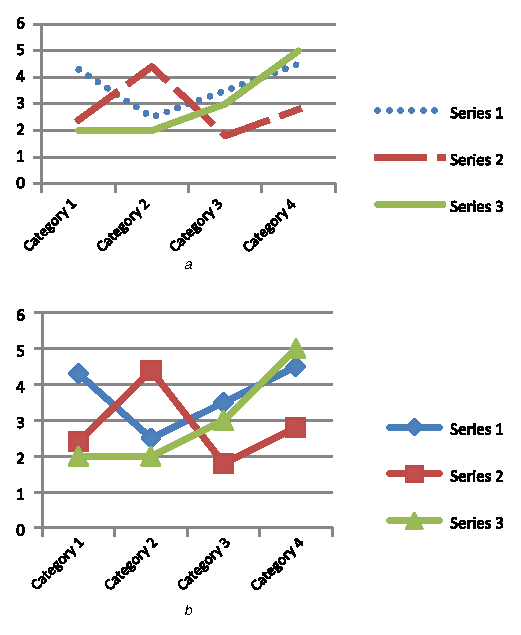
\includegraphics{sample_1.eps}}
\caption{Sample graph with blue (dotted), green (solid) and red (dashed) lines
\figfooter{a}{Subfigure 1}
\figfooter{b}{Subfigure 2}\label{fig1}}
\end{figure}

\begin{figure*}[!b]
\centering{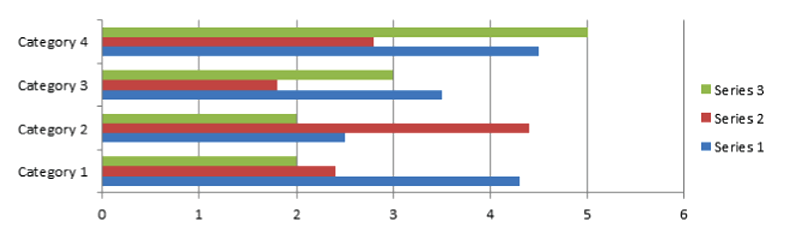
\includegraphics{sample_2.eps}}
\caption{Sample graph spaning two columns\label{fig2}}
\end{figure*}

\subsubsection{Second Level Headings}\label{subsubsec5.3.2}

The second level section headings should be in italic font
(i.e. ``\textit{2.3 Section Headings}''. The paragraph
should start on a new line.

\subsubsection{Third Level Headings}\label{subsubsec5.3.3}

The third level section headings should also be in italic
font but should end with a colon (:). The text for that
section should run on and not start as a new paragraph.


\section{Figures}\label{sec6}

Figures will be reproduced exactly as supplied, with no
redrawing or relabelling. It is therefore imperative that
the supplied figures are of the highest possible quality.
The preferred format is encapsulated postscript (.eps) for
line figures and .tif for halftone figures with a minimum
resolution of 300\,dpi (dots per inch). With larger
figures, please note that the editorial office may contact
you to revise them to ensure they do not exceed half of a
page, or so that they fill the entire page. This is because
figures between these two lengths may negatively impact
production later.

Graphics may be full colour but please make sure that they
are appropriate for print (black and white) and online
(colour) publication. For example lines graphs should be
colour and use dotted or dashed lines, or shapes to
distinguish them apart in print (see Fig.~\ref{fig1}). Each
figure should be explicitly referred to in numerical order.
A maximum of four subfigures will be allowed per figure.

Please note that IET typeset format is to float figures to
the top or bottom of a page, they cannot appear within the
main body,  interrupting the text.

Figures can span two columns but cannot exceed 17.5\,cm in
width (see Fig.~\ref{fig2}).

%Figures and their subfigures should be treated as a static
%image and should not fall onto other pages or columns.

\begin{table}[!b]
\processtable{Example table\label{tab1}}
{\begin{tabular*}{20pc}{@{\extracolsep{\fill}}lll@{}}\toprule
Column  &Column  & Column heading \\
heading  &heading two &  three \\
\midrule
Row 1a  &Row 1b  &Row 1c \\
Row 2a  &Row 2b  &Row 2c \\
Row 3a  &Row 3b  & Row 3c \\
Row 4a  &Row 4b  &Row 4c \\
Row 5a  &Row 5b  &Row 5c \\
Row 6a  & Row 6b  & Row 6c \\
\botrule
\end{tabular*}}{}
\end{table}

\subsection{Figure Captions}\label{subsec6.1}

Figure captions must be below the figure, in 10\,pt italic
font and should ideally consist of one sentence. If a
figure has subfigures, all subfigures should also have a
caption and should be identified by letters, e.g. $a$, $b$,
$c$, as shown above.

\section{Tables}\label{sec7}

Tables should be formatted as shown in Table~\ref{tab1}
with no column lines unless needed to clarify the content
of the table. Row lines can be used to distinguish the
column headings from the content of the table. Any tables
larger than half a page should be placed in an appendix and
the appendix cited within the main body of text eg. ``see
Appendix 1 for table of results''.

If the table has four or five columns it should span the
whole width of the page. These should also float to the top
or bottom of the page instead of breaking up the main text.

\subsection{Table Captions}\label{subsec7.1}

Tables must be numbered and cited within the text in strict
numerical order. Table captions must be above the table and
in 10\,pt font

\section{Mathematics and equations}\label{sec8}

When writing mathematics, avoid confusion between
characters that could be mistaken for one another, e.g. the
letter 'l' and the number one.

\setcounter{equation}{2}

\begin{figure*}[!t]
\begin{equation}
f(x)  = a_0 + \sum_{n=1}^\infty
\left( {a_n \cos \frac{n\pi x}{L}+b_n \sin \frac{n\pi
x}{L}} \right)+f(x) =a_0 +\sum_{n=1}^\infty \left({a_n \cos \frac{n\pi x}{L}+b_n
\sin \frac{n\pi x}{L}} \right) \label{eq3}
\end{equation}
\noindent\rule{\textwidth}{.5pt}%\vskip3pt
\end{figure*}

\setcounter{equation}{0}

Refer to equations using round brackets, e.g. (\ref{eq1})
followed by (\ref{eq2}).
\begin{align}
A & = \pi r^2 \label{eq1}\\
\cos \alpha +\frac{\Delta y}{\Delta x}\cos \beta & =2\cos
\frac{1}{2}\left( {\alpha +\beta } \right)\cos \frac{1}{2} \sum
\left({\alpha \frac{dy}{dx}-\beta}\right)\label{eq2}
\end{align}
Equations should be capable of fitting into a two-column
print format. If they do not fit into one column they
should be floated to the bottom of the page or top of the
next and cited in the text by "(see (3))". All large
equations must be numbered in order to avoid confusion
between floated equations and they cannot exceed a width of
17.5cm.

Vectors and matrices should be in bold italic and variables
in italic.

If your paper contains superscripts or subscripts, take
special care to ensure that the positioning of the
characters is unambiguous.

Exponential expressions should be written using superscript
notation, i.e. $5 \times 10^{3}$ not 5E03. A multiplication
sign should be used, not a dot.

Inline equations can be used but if the equation is longer
than a line it will need to be broken up in a suitable
location to ensure the line spacing is not too
large $a^2+b^2=c^2$.

\section{Page Numbers and Footers}\label{sec9}

Page numbers should be used on all pages. Footers are not
in IET's house style so must not be used. If they are used
they will be moved to within the text at the typesetting
stage.

\section{Conclusion}\label{sec10}

Submissions should always include the following sections:
an abstract; an introduction; a conclusion and a references
section. If any of the above sections are not included the
paper will be unsubmitted and you will be asked to add the
relevant section.

\section{Acknowledgments}\label{sec11}

Acknowledgements should be placed after the conclusion and before the
references section. This is where reference to any grant numbers or
supporting bodies should be included. The funding information should also be
entered into the first submission step on Manuscript Central which collects
Fundref information [4].

Please note that the IET does not include author biographies in published
papers.


\section{References}\label{sec12}

An average research paper should reference between 20 and 30 works, the bulk
of which should be recently published (i.e. within the last five years)
leading-edge articles in the field, preferably from top journals or
conferences. You should compare your own findings to this recent research
and demonstrate how your work improves on it in order to demonstrate that
your work shows a significant advance over the state of the art -- a
pre-requisite for publication in IET Research Journals.

Please note that tables, figures and equations should not appear in the
middle of the references. If this happens white space will be introduced to
avoid items appearing in the references.

\subsection{Referencing Style}\label{subsec12.1}

You should number your references sequentially throughout the text, and each
reference should be individually numbered and enclosed in square brackets
(e.g. [1]).

Please ensure that all references in the Reference list are cited in the
text and vice versa. Failure to do so may cause delays in the production of
your article.

Please also ensure that you provide as much information as possible to allow
the reader to locate the article concerned. This is particularly important
for articles appearing in conferences, workshops and books that may not
appear in journal databases.

Do not include references for papers that have been submitted and not
accepted for publication. Papers that have been accepted for publication are
allowed as long as all information is provided.

Please provide all author name(s) and initials, title of the paper, date
published, title of the journal or book, volume number, editors (if any),
and finally the page range. For books and conferences, the town of
publication and publisher (in parentheses) should also be given.

If the number of authors on a reference is greater than three please list
the first three authors followed by \textit{et~al.} The reference list should be uninterrupted by figures, tables or equations.

%Nothing should interrupt the references.

\section*{Example References}\label{sec13}

\subsection{Websites}\label{subsec13.1}

\begin{enumerate}
\item[{[1]}] `Author Guide - IET Research Journals',
http://digital-library.theiet.org/journals/author-guide, accessed 27
November 2014\vspace*{6pt}

\item[{[2]}] `Research journal length policy',
http://digital-library.theiet.org/ files/research\_journals\_length\_policy.pdf,
accessed 27 November 2014
\end{enumerate}

\subsection{Patent}\label{subsec13.2}

\begin{enumerate}
\item[{[3]}] `ORCID: Connecting research and researchers', http://orcid.org/,
accessed 3 December 2014\vspace*{6pt}

\item[{[4]}]
`Fundref', http://www.crossref.org/fundref/, accessed 4 December 2014
\end{enumerate}

\subsection{Journal articles}\label{subsec13.3}

\begin{enumerate}
\item[{[5]}] Smith, T., Jones, M.: 'The title of the paper', IET Syst. Biol., 2007,
1, (2), pp. 1--7\vspace*{6pt}

\item[{[6]}] Borwn, L., Thomas, H., James, C.,~et al.:'The title of the paper, IET
Communications, 2012, 6, (5), pp 125-138
\end{enumerate}

\subsection{Conference Paper}\label{subsec13.4}

\begin{enumerate}
\item[{[7]}]
Jones, L., Brown, D.: 'The title of the conference paper'. Proc. Int.
Conf. Systems Biology, Stockholm, Sweden, May 2006, pp. 1--7
\end{enumerate}

\subsection{Book, book chapter and manual}\label{subsec13.5}

\begin{enumerate}
\item[{[8]}] Hodges, A., Smith, N.: 'The title of the book chapter', in Brown, S.
(Ed.): 'Handbook of Systems Biology' (IEE Press, 2004, 1st edn.), pp. 1--7\vspace*{6pt}

\item[{[9]}]
Harrison, E.A., and Abbott, C.: 'The title of the book' (XYZ Press,
2005, 2nd edn. 2006)
\end{enumerate}

\subsection{Report}\label{subsec13.6}

\begin{enumerate}
\item[{[10]}] IET., 'Report Title' (Publisher, 2013), pp. 1-5\vspace*{6pt}

\item[{[11]}] Brown, F.: 'The title of the patent (if available)'. British Patent
123456, July\vadjust{\pagebreak} 2004

\item[{[12]}] Smith, D., Hodges, J.: British Patent Application 98765, 1925
\end{enumerate}

\subsection{Thesis}\label{subsec13.7}

\begin{enumerate}
\item[{[13]}]
Abbott, N.L.: 'The title of the thesis'. PhD thesis, XYZ University,
2005
\end{enumerate}

\subsection{Standard}\label{subsec13.8}

\begin{enumerate}
\item[{[14]}] BS1234: 'The title of the standard', 2006
\end{enumerate}

\begin{table}[!h]
\fwprocesstable{Example of large table\label{tab2}}
{\begin{tabular*}{\textwidth}{@{\extracolsep{\fill}}lccc}\toprule
Column heading 1 &Column heading 2 & Column heading 3  & Column heading 4\\
\midrule
Result 1 &123 &123 & 123 \\
Result 2 &123 &123 &123 \\
Result 3 &123 &123 &123 \\
Result 4 &123 &123 &123 \\
Result 5 &123 &123 &123 \\
Result 6 &123 &123 &123 \\
Result 7 &123 &123 &123 \\
Result 8 &123 &123 &123 \\
\botrule
\end{tabular*}}{}
\end{table}

\vfill\pagebreak

\section{Appendices}\label{sec14}

Additional material, e.g. mathematical derivations, tables and figures
larger than half a page that may interrupt the flow of your paper's argument
should form a separate Appendix section (see Table~\ref{tab2}). Do not, however, use
appendices to lengthen your article unnecessarily as this section is
included in the word count. If the material can be found in another work,
cite this work rather than reproduce~it.
The appendix section should be in double column format, and come after the references.

\end{document}
